\chapter{Project Framework}

\section{Introduction}
This chapter presents a general overview of this end-of-studies project. It lays out the context and influences which made it relevant in current settings.
First, it describes the background and sequence of developments that brought much of the employed technologies into existence. Next, it introduces the hosting company and discusses its necessity for such a novel solution. And finally, it lists the pursued objectives and innovations which address the insufficiencies of existing solutions.

\section{Background}
Business Knowledge is both integral and proprietary for any enterprise. The contents of private documents are useful for internal employees who are constantly consuming it to accomplish their workstreams. It becomes evident when considering that modern software development and network infrastructure deployment (among many other fields) are often based on exploring exhaustive documentation and lengthy research papers. Paradoxically, this upfront research and learning introduce a sort of bottleneck, requiring much time before a new project gets initiated. In most cases, a further looking up for previously reviewed information is often required. Accelerating delivery, however, remains a key aspiration for organizations seeking a competitive edge. This together emphasizes the need to consider and propose innovative solutions which would help reduce the preliminary requirements and achieve faster delivery cycles.\medskip\newline
In line with this discussion, it is worth highlighting the evolving landscape of web search in the contemporary era. We used to input a query into a search engine (e.g. Google) and it would look through its indexed webpages and then return a list of the most relevant pages which we would then read until we have a satisfying answer. This paradigm has veered towards generative AI chatbot solutions, like ChatGPT, Copilot and Gemini, which leverage Machine Learning algorithms to mimic the natural language understanding capability of humans to generate short and accurate answers based on public information and the open web.\smallskip\newline
Auspiciously, the underlying technology that empower this kind of chatbots is discrete from their corresponding platforms, i.e., it can be integrated in other projects as a library or a software component rather than being exclusive to their native applications, which makes customizing their functioning and augmenting their knowledge possible. This presents an interesting theme for an internship project which attempts to build upon these technologies to provide a much needed solution for an entreprise with many activities and projects to accomplish and for a data science student aspiring to continuously learn the newest trends in AI and Machine Learning.

\section{Hosting Company}
The hosting of this project was managed by Standard Sharing Software (3S).\smallskip
\begin{figure}[H]
    \centering
    
\includegraphics[width=0.4\linewidth]{./figures/logo_3S.png}
    \caption{Standard Sharing Software logo}
\end{figure}
3S Group, founded in 1988 with the mission of transforming the Tunisian technological landscape, is a leading company in Tunisia specializing in the integration of IT infrastructures and the provisioning of advanced technological solutions. The group brings together more than 650 employees spread across 16 separate affiliates, each specialized in different cutting-edge technologies, covering a wide range of sectors including the integration of IT infrastructures, the provisioning of internet services, the edition of ERP solutions, and the management of multichannel call centers.\newline
It is based in Montplaisir, Tunis, Tunisia (headquarters), and in Charguia 1, Tunis (the office where this internship was conducted), with different teams specializing in Network and Telecommunication infrastructures, Cyber security, Cloud Computing and Software. This project was organized and executed in the Cloud and Software department of the company yet close collaboration with these different units was required since they constitute the target users of this project.\newline
3S Group's work culture helped the success of this project with its core values of commitment, excellence, innovation and teamwork, which were reflected during the whole duration of this internship, from project initialization until delivery, as evidenced by the organizers's relentless dedication to meeting project deadlines, the pursuit of using innovative tools, the collaborative problem-solving approach, and the unwavering commitment to delivering exceptional results.

\section{Study of the Existing}
\subsection{Problem Statement}
Traditional enterprise search engines, including those currently utilized by 3S employees, face significant limitations in effectively comprehending the context of user queries and the nuances of human language. These systems often rely on exact text matching, which fails to capture the semantic meaning behind queries, leading to inefficient and incomplete retrieval of information.\medskip\newline
Even with the advent of AI tools that solve these Natural Language Processing (NLP) tasks, accessing and leveraging large volumes of enterprise data remains a challenge for such proprietary systems. The complexity is further compounded by increasing regulatory scrutiny on AI products, driven by concerns over privacy and copyright infringement.\smallskip\newline
While such regulations are essential for protecting sensitive information and ensuring compliance with legal standards, they also pose obstacles to integrating advanced AI tools into enterprise environments. This underscores the need for companies to develop their own tailored solutions to fully harness recent AI advancements while navigating regulatory constraints.\bigskip\newline
A Retrieval-Augmented Generation (RAG) system addresses these challenges by combining state-of-the-art retrieval techniques with large language models (LLMs). This system can enhance employees' access to enterprise data by accurately locating relevant information from vast datasets and presenting it in a coherent, contextually appropriate manner. Ultimately, this approach empowers employees to make better-informed decisions, boosts productivity, and ensures compliance with privacy and copyright standards.
\subsection{Criticism of the Existing}
While there are some systems which attempt to resolve the same issues as our project, these solutions come with some inadequacies.
The table below identifies these solutions and their limitations in order to build upon them.
\begin{table}[H]
    \centering
    \begin{tabular}{|c|c|c|c|}
        \toprule
        \textcolor{darkgray}{\textbf{\makecell{Solution}}}  & \textbf{\makecell{LLM                                                                                               \\Chatbots}}                                     & \textbf{\makecell{NotebookLM}}                                       & \textbf{\makecell{Verba}}                                             \\
        \midrule
        \textcolor{darkgray}{\textbf{\makecell{Developer}}} & \makecell{Google, OpenAI                                                                                            \\and Microsoft}                                 & Google                                                    & Weaviate                                                   \\
        \midrule
        \textcolor{darkgray}{\textbf{\makecell{RAG-based                                                                                                                          \\ (with persistent storage)}}} & \textcolor{red}{\ding{56}}        & \textcolor{green}{\ding{52}}                                & \textcolor{green}{\ding{52}}  / \textcolor{red}{\ding{56}} \\
        \midrule
        \textcolor{darkgray}{\textbf{\makecell{Enterprise                                                                                                                         \\focused}}} & \textcolor{red}{\ding{56}}                                & \textcolor{red}{\ding{56}}                                & \textcolor{green}{\ding{52}}  / \textcolor{red}{\ding{56}} \\
        \midrule
        \textcolor{darkgray}{\textbf{Extensible}}           & \textcolor{green}{\ding{52}} / \textcolor{red}{\ding{56}} & \textcolor{red}{\ding{56}} & \textcolor{red}{\ding{56}} \\
        \midrule
        \textcolor{darkgray}{\textbf{\makecell{Multiple                                                                                                                           \\LLMs}}}      & \textcolor{red}{\ding{56}}                                & \textcolor{red}{\ding{56}}                                & \textcolor{green}{\ding{52}}                               \\
        \midrule
        \textcolor{darkgray}{\textbf{\makecell{User-LLM                                                                                                                           \\feedback}}}  & \textcolor{green}{\ding{52}} & \textcolor{red}{\ding{56}} / \textcolor{green}{\ding{52}} & \textcolor{red}{\ding{56}}                                 \\
        \midrule
        \textcolor{darkgray}{\textbf{\makecell{Stable                                                                                                                             \\ (Not experimental)}}} & \textcolor{green}{\ding{52}} & \textcolor{red}{\ding{56}}                                & \textcolor{red}{\ding{56}}                                 \\
        \bottomrule
    \end{tabular}
    \caption{Comparison of existing solutions}
    \begin{flushleft}
        \par The table above provides a comparative review of some of the most suitable similar solutions (AI chatbots, NotebookLM, and Verba), highlighting their features and limitations.\newline "RAG-based" refers to whether or not the solution automatically retrieves relevant passages from a knowledge base, rather than passing the context manually each time. "Entreprise focused" suggests that the solution was designed to address entreprise requirements such as managing and sharing different knowledge base partitions for different teams. "Extensible" means that the solution can be further tweaked or developed to modify and add new features. "Multiple LLMs" indicates that the solution provides multiple models generating responses each time. "User-LLM feedback" signifies the ability for users to provide feedback for generated responses, which can be used to enhance future behavior. "Stable" refers to stability of the product.
    \end{flushleft}
\end{table}
In general, one can utilize any ready-to-use LLM-powered chatbot (e.g. ChatGPT, Microsoft Copilot, Google Gemini, and many others). But these solutions, even though allowing document-answering, don't come with document persistence, which means by leaving the chat, the documents are gone unless re-uploaded.\smallskip\newline
Google is currently experimenting with a new solution (NotebookLM) which allows exactly that by connecting to cloud-hosted documents, in addition to methods allowing to upload local files and webpage content from URLs. Nonetheless, this falls short for enterprise usage as it is intended for casual use cases (e.g. note taking, document editing suggestions and personal project research) rather than question-answering from a large knowledge base and does not provide features to share documents between different users.\smallskip\newline
On the other hand, Weaviate, a company behind a vector store implementation, maintains \href{https://github.com/weaviate/Verba}{a repository on GitHub} which addresses the same objectives as this project. Their solution, called Verba, is a well-organized open-source project that can be easily deployed on-premises or in a cloud environment. However, several challenges need to be addressed before a company can use and adapt it to their specific needs: customization is difficult, if not impossible, given that the project depends on many packages they developed or contributed to (goldenverba, weaviate, ...), requiring many API keys from various providers (vector database, LLMs, cloud providers, etc...), in addition to the inability to create and manage different databases for different teams.\smallskip\newline
This scarcity and inadequacy of available solutions raises the need to design and develop a custom product suitable for the specific needs and requirements set up by individual enterprises, which are discussed in the following section for our case.

\section{Proposed Solution}
This project aims to develop a novel search functionality that leverages retrieval-augmented generation techniques to deliver insightful results for enterprise data, by addressing general-purpose large language models' limitations, which can be summed up in data confinement to training phase and private data access. The system will prioritize the following objectives.
\subsection{Objectives}
\begin{itemize}
    \item Enhance AI-generated responses with External Knowledge: Retrieve relevant passages from a curated enterprise knowledge base each time a LLM is prompted to improve its factual grounding and reduce the risk of hallucinating.
    \item Flexible Data Ingestion and Organization: Implement diverse methods for multi-source, format-agnostic file content and document indexing into manageable and domain-specific vector databases to tailor to enterprise needs and potential evolution.
    \item Diverse Answering Options: Allow the selection from a list of various Large Language Models for answering and just-in-time (of generating responses) data scraping to diversify and improve results each time.
    \item User-Driven Feedback: Integrate a mechanism for providing user feedback for LLM-generated responses which can be used to rank future results and further train and improve LLMs (when supported).
    \item Leverage RAG-based metrics for evaluation: Employ retrieval-augmented generation evaluation metrics to assess the quality of pipeline stages' results (retrieval quality/accuracy, context-generation consistency, answer relevancy)
\end{itemize}
\subsection{Significance of RAG}
RAG technology comes with many benefits for businesses in the context of leveraging generative AI models for content searching:
\begin{itemize}
    \item Private and up-to-date data: Even with the best performing generative AI chatbots, it is challenging to maintain relevancy in an enterprise environment. By allowing AI models to connect to external knowledge bases and personal data, much more relevant results can be achieved.
    \item Cost-effective: Even with the availability of open-source LLMs and cloud-based FMs (Foundational Models), the computational and financial costs of re-training such models on domain-specific or private data can be high. By circumventing the re-training phase of LLMs, a huge gain can be brought off using this technique.
    \item More control and customization: It is easy for developers to customize RAG pipelines: Adapting to changing requirements and sources of information, troubleshooting model performance and results, restricting access to some information for authorized users, etc...
    \item User trust: By enabling user choices and interference in the overall process of RAG, users can look up how their choices in information sources and LLM selections directly affect the system's performance and results.
\end{itemize}
In many ways, RAG techniques, when combined with an effective Prompt Engineering approach, provide an alternative framework to re-training or fine-tuning with better adaptability and performance on knowledge-intensive tasks. This is because it is difficult for LLMs to capture new factual information through unsupervised fine-tuning. The following figure demonstrates the effectiveness of a RAG pipeline when a model does not have access to recent information.
\begin{figure}[H]
    \centering
    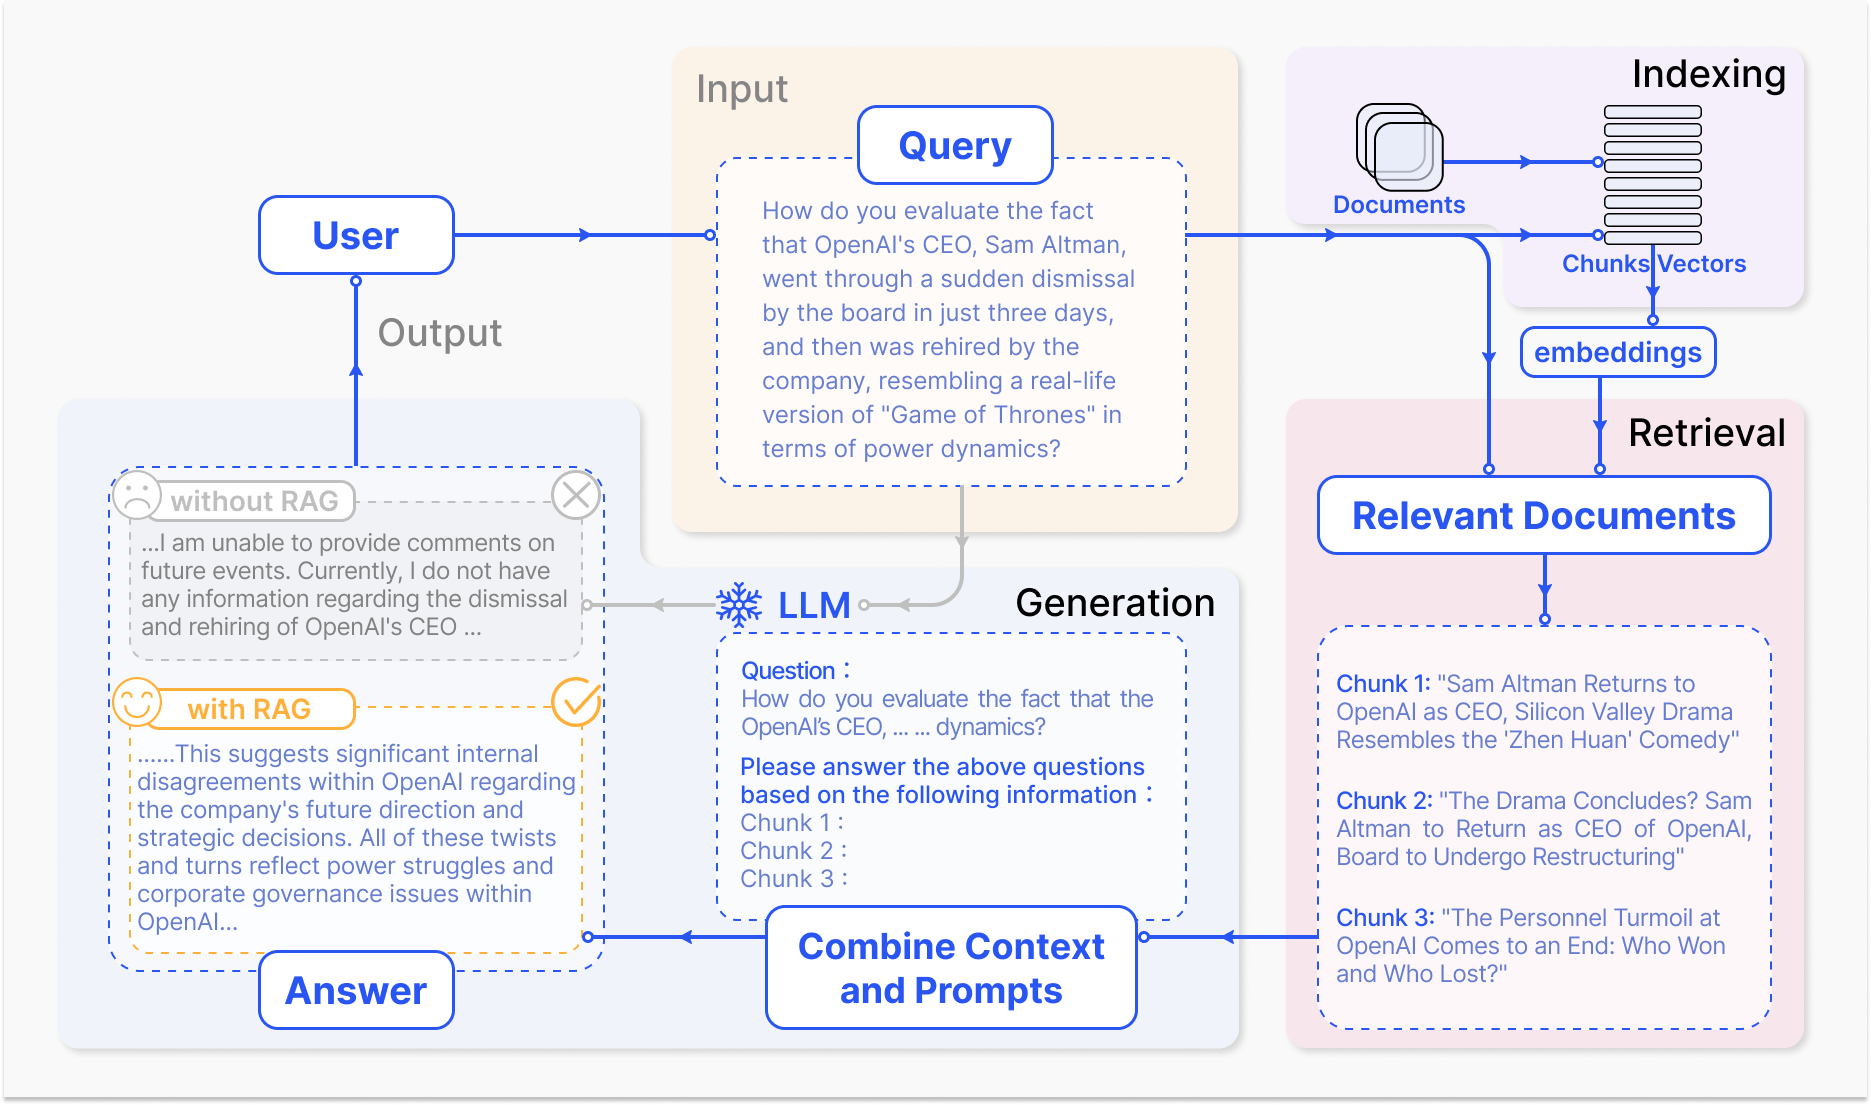
\includegraphics[width=\linewidth]{./figures/RAG_case.png}
    \caption{An illustration of a RAG pipeline in work \cite{ragforllmsasurvey}}
    \begin{flushleft}
        \small A comparative representation between a simple LLM and a RAG process applied to question answering. Prompting the LLM directly resulted in its inability to provide a suitable answer because its does not have access to new information. The RAG process, on the other hand, has successfully identified the relevant information from the knowledge base and made the LLM capable of generating a factual response.
    \end{flushleft}
\end{figure}
\subsection{Significance of the Solution}
The proposed Generative AI solution would help employees find answers from enterprise knowledge without having to browse vast amounts of documents. This is enabled by augmenting LLM knowledge using the techniques of retrieval-augmented generation and prompt engineering for context precision. It would also allow them to interfere in the steps of answer-generation by providing ways to customize the external knowledge base and conduct online researching, powered by traditional search engines and generative AI researching tools, through a unified interface.\medskip\newline
From an educational perspective, this project presents a valuable opportunity to gain expertise on some of the most capable ML models and personalize and extend their functioning. The anticipated learning outcomes of accomplishing this project include an enhanced perception of large models' parameters and how they affect performance, picking up prompt engineering techniques, planning out and implementing RAG pipelines that tailor to complex requirements, using both local and cloud components, in addition to developing various data scraping methods.

\section{Conclusion}
This first chapter has given grounds for the development of the proposed solution for the hosting company, by presenting the limitations of existing solutions and identifying key objectives to implement during the internship.\newline
In the following chapter, we will break down the project's requirements and select a management strategy, in addition to identifying tasks and setting up deadlines.